#import "@local/bootlin:0.1.0": *

#import "@local/bootlin-yocto:0.1.0": *

#import "@local/bootlin-utils:0.1.0": *

#import "../../typst/local/themeBootlin.typ": *

#import "../../typst/local/common.typ": *

#show: bootlin-theme.with( aspect-ratio: "16-9", config-common(handout: "handout" in sys.inputs and sys.inputs.handout == "1", ))

#show raw.where(block: true): set block(fill: luma(240), inset: 1em, radius: 0.5em, width: 100\%)

#show raw.where(block: true): set text(size: 11pt)

#show raw.where(block: false): r => text(fill: color-link)[#r]

#show raw.where(lang: "c", block: true): set block(fill: luma(240), inset: 0.4em, radius: 0.5em, width: 95\%, breakable: true, above: 12pt, below: 12pt)

#show raw.where(lang: "c", block: true): set text(11pt)

#show raw.where(lang: "console", block: true):set block(fill: luma(240), inset: 0.4em, radius: 0.5em, width: 95\%, breakable: true, above: 6pt)

#show raw.where(lang:"console", block: true): set text(12pt)

 == TF-A: Trusted Firmware

=== {Concept of FIP}
  \begin{itemize}
  \item FIP = {\em Firmware Image Package}
  \item Concept specific to TF-A
  \item {\em packaging format used by TF-A to package firmware images
      in a single binary}
  \item Typically used to bundle the BL33, i.e. the U-Boot bootloader
    that will be loaded by TF-A.
  \item \url{https://trustedfirmware-a.readthedocs.io/en/latest/getting_started/tools-build.html}
  \item \url{https://wiki.st.com/stm32mpu/wiki/How_to_configure_TF-A_FIP}
  \end{itemize}


=== {Configuring TF-A}
  \begin{itemize}
  \item TF-A does not use {\em Kconfig} for configuration
  \item All the configuration is based on variables passed on the
    `make` command line
  \item Most variables are documented at:
    \url{https://trustedfirmware-a.readthedocs.io/en/latest/getting_started/build-options.html}
  \end{itemize}


=== {Configure TF-A: important variables}
  \begin{itemize}
  \item `CROSS_COMPILE`, cross-compiler prefix
  \item `ARCH`, CPU architecture: `aarch32` or `aarch64`
  \item `ARM_ARCH_MAJOR`, `7` for ARMv7, `8` for ARMv8
  \item `PLAT`, SoC family, any directory name in `plat`
    that contains `platform.mk`
  \item `AARCH32_SP`, the Secure Payload, specific to
    ARMv7. Either OP-TEE or the built-in {\em SP-MIN} provided by TF-A
  \item `DTB_FILE_NAME`, path to the Device Tree describing our board
  \item `BL33`, path to the second stage bootloader, usually
    U-Boot, to include in the FIP image
  \item Specific to STM32MP1
    \begin{itemize}
    \item `BL33_CFG`, path to the U-Boot Device Tree
    \item `STM32MP_SDMMC=1`, enable support for SD card/eMMC in TF-A
    \end{itemize}
  \end{itemize}


=== [fragile]{Building TF-A for STM32MP1}
  \begin{block}{}
    {\footnotesize
\begin{verbatim}
$ make CROSS_COMPILE=arm-linux- \
        ARM_ARCH_MAJOR=7 \
        ARCH=aarch32 \
        PLAT=stm32mp1 \
        AARCH32_SP=sp_min \
        DTB_FILE_NAME=stm32mp157a-dk1.dtb \
        BL33=/path/to/u-boot/u-boot-nodtb.bin \
        BL33_CFG=/path/to/u-boot/u-boot.dtb \
        STM32MP_SDMMC=1 \
        fip all
\end{verbatim}
    }
  \end{block}

  Build results in `build/stm32mp1/release`. Important files:

  \begin{itemize}
  \item `tf-a-stm32mp157a-dk1.stm32`, TF-A itself
  \item `fip.bin`, the FIP image, containing U-Boot and other
    elements
  \end{itemize}


=== [fragile]{FIP image contents}
  \begin{block}{fiptool info}
    {\footnotesize
\begin{verbatim}
$ ./tools/fiptool/fiptool info build/stm32mp1/release/fip.bin Secure Payload BL32 (Trusted OS): offset=0x100, size=0x8AEC, cmdline="--tos-fw"
Non-Trusted Firmware BL33: offset=0x8BEC, size=0xECE6C, cmdline="--nt-fw"
FW_CONFIG: offset=0xF5A58, size=0x226, cmdline="--fw-config"
HW_CONFIG: offset=0xF5C7E, size=0x16A98, cmdline="--hw-config"
TOS_FW_CONFIG: offset=0x10C716, size=0x3CF6, cmdline="--tos-fw-config"
\end{verbatim}
    }
  \end{block}


=== {STM32MP1 partition layout}
  
#table(columns: (50\%, 50\%), stroke: none,
[
  \begin{center}
    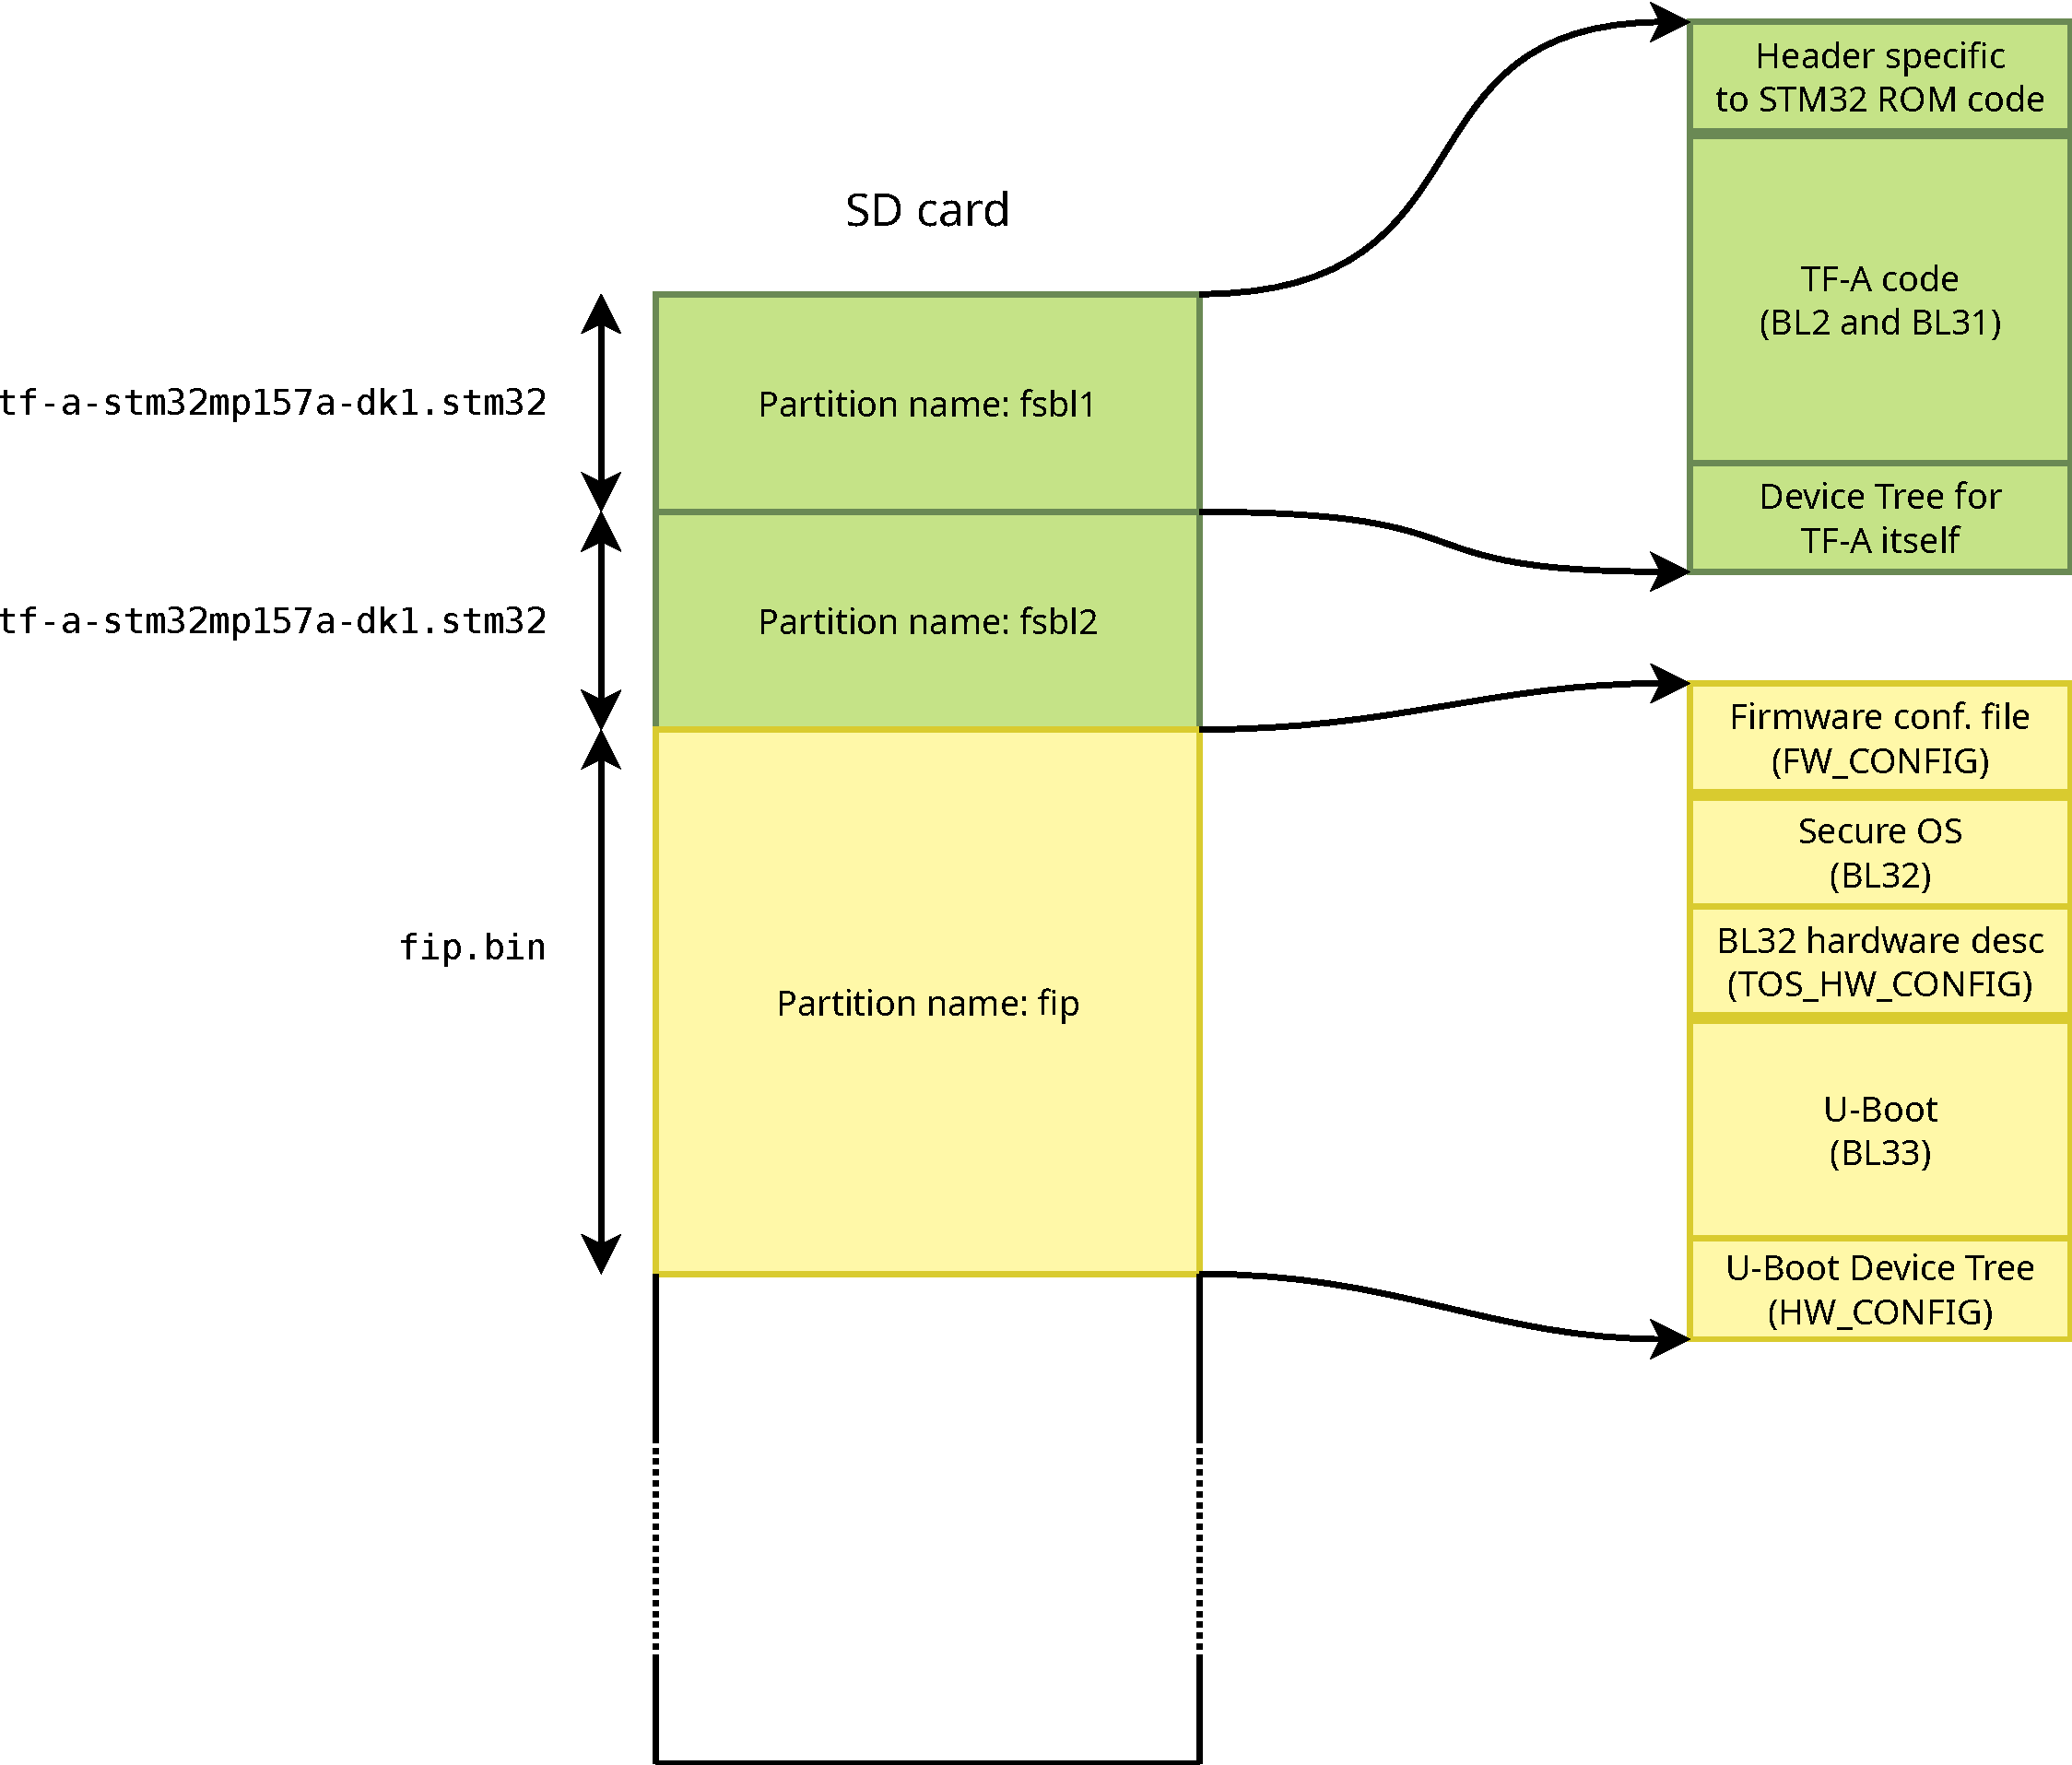
\includegraphics[width=0.9\textwidth]{slides/sysdev-bootloaders-tf-a/stm32mp1-tfa.pdf}
  \end{center}
  \column{0.4\textwidth}
  \small Reminder: boot sequence with TF-A on STM32MP1
  \begin{center}
    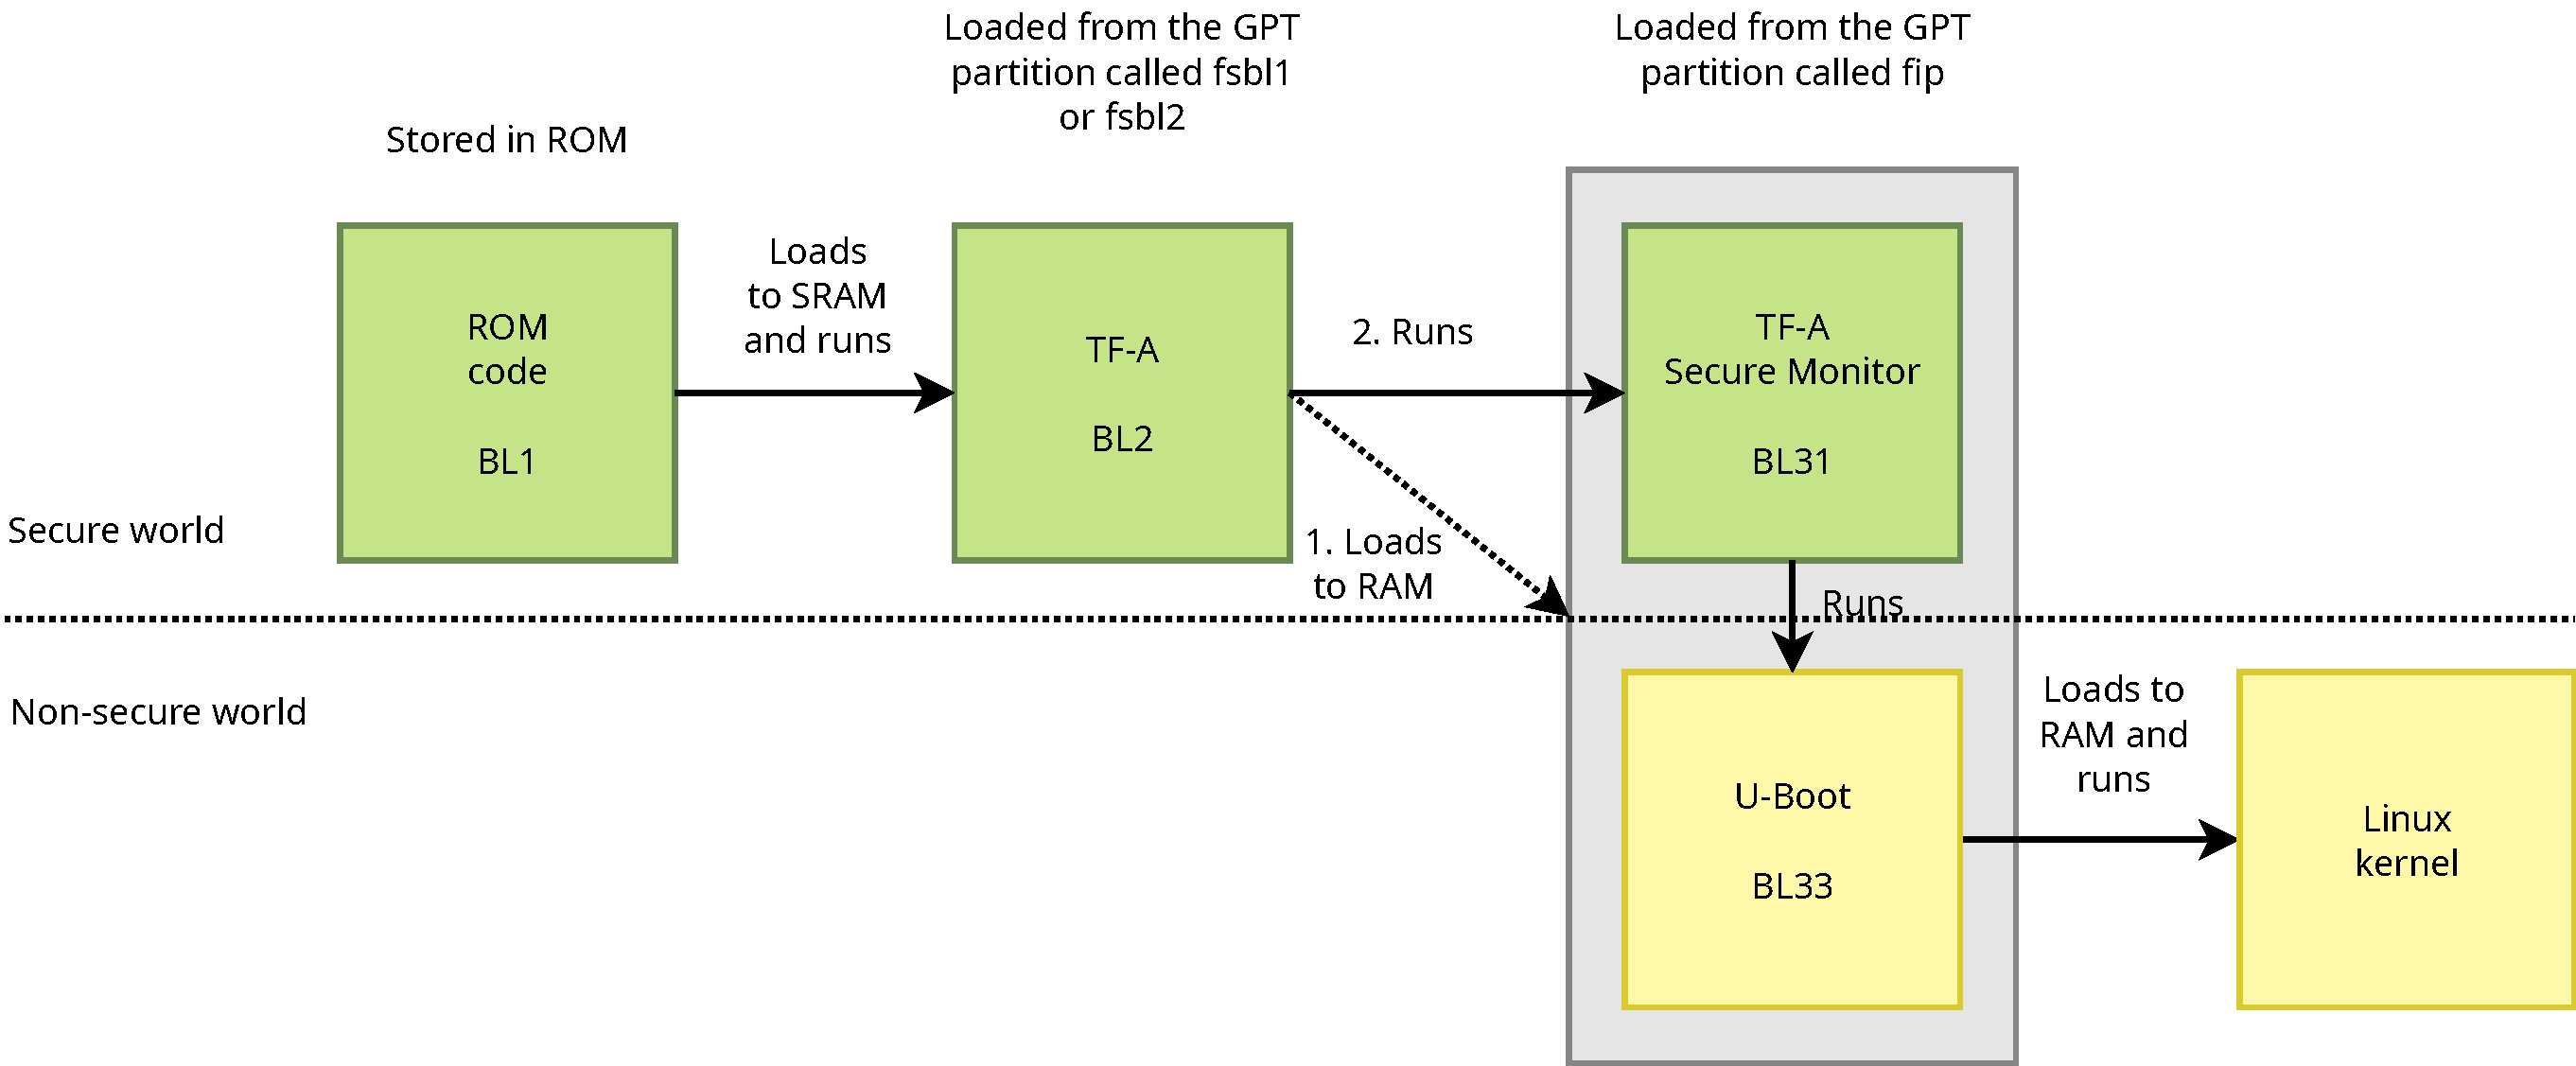
\includegraphics[width=\textwidth]{common/sequence-stm32mp1.pdf}
  \end{center}
  \\]


=== {AM62x (BeaglePlay) partition layout}
  
#table(columns: (50\%, 50\%), stroke: none,
[
  \begin{center}
    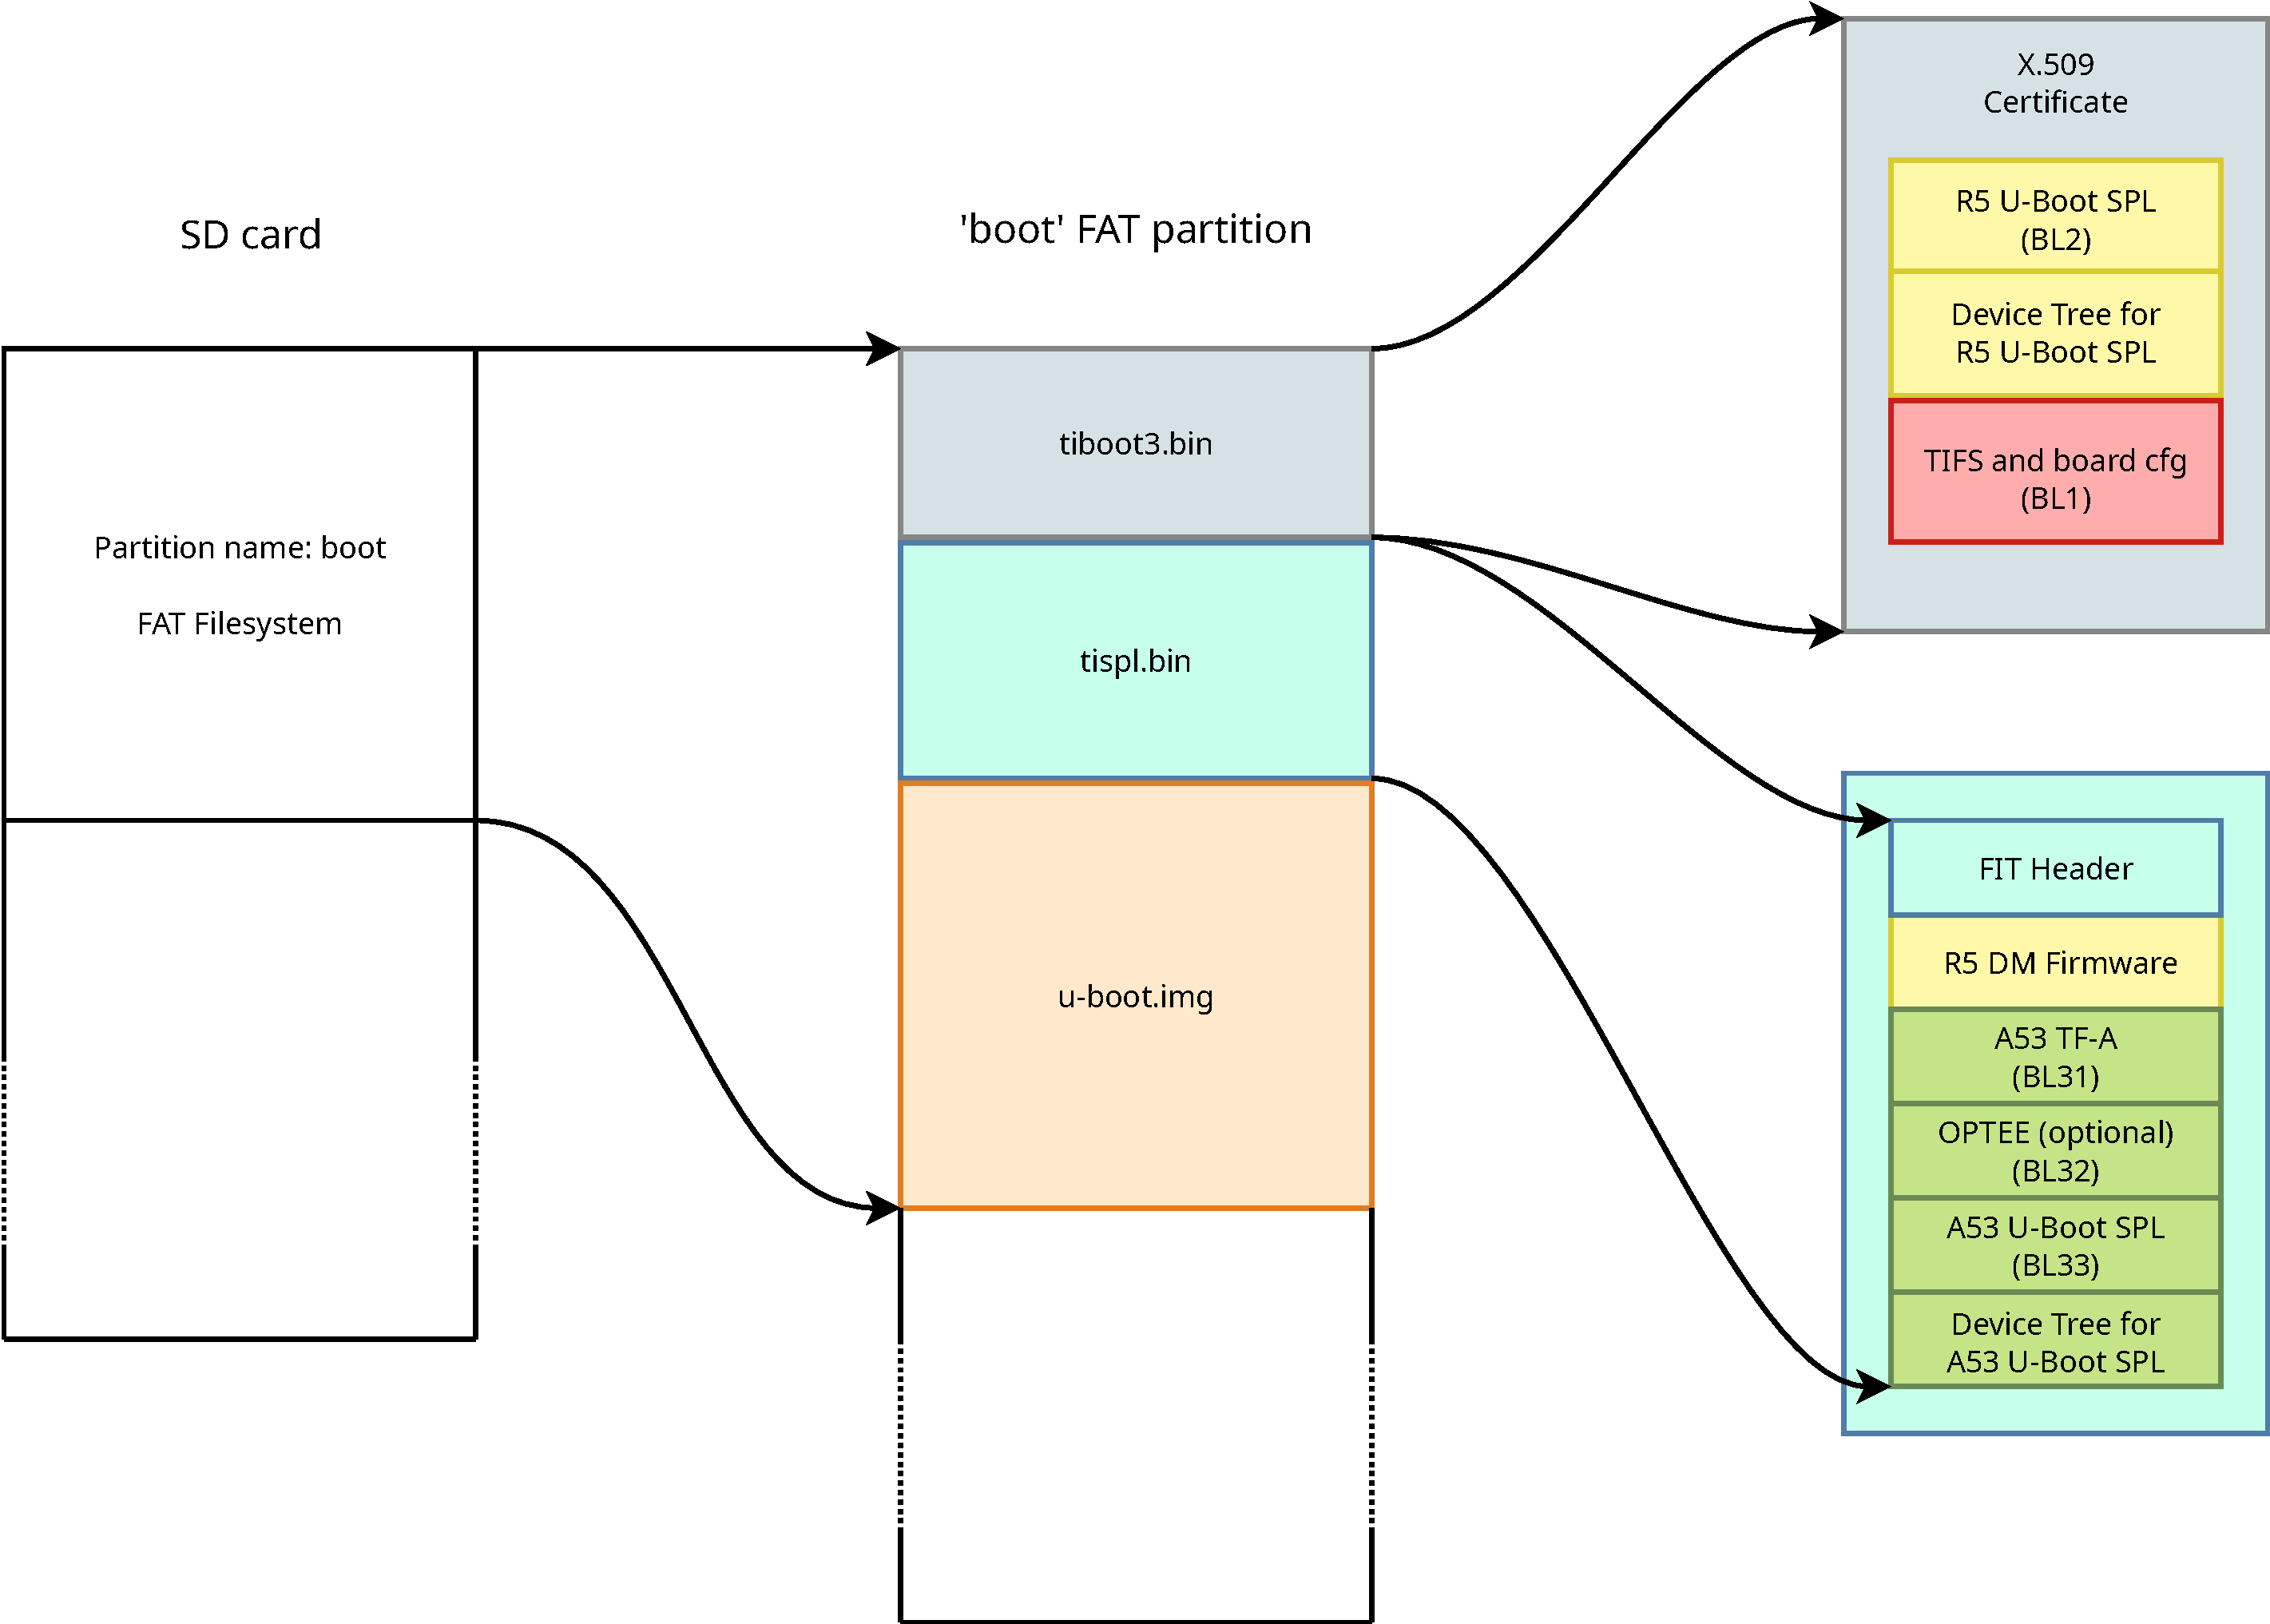
\includegraphics[width=0.9\textwidth]{slides/sysdev-bootloaders-tf-a/am62x-tfa.pdf}
  \end{center}
  \column{0.4\textwidth}
  \small Reminder: boot sequence with TF-A on AM62x
  \begin{center}
    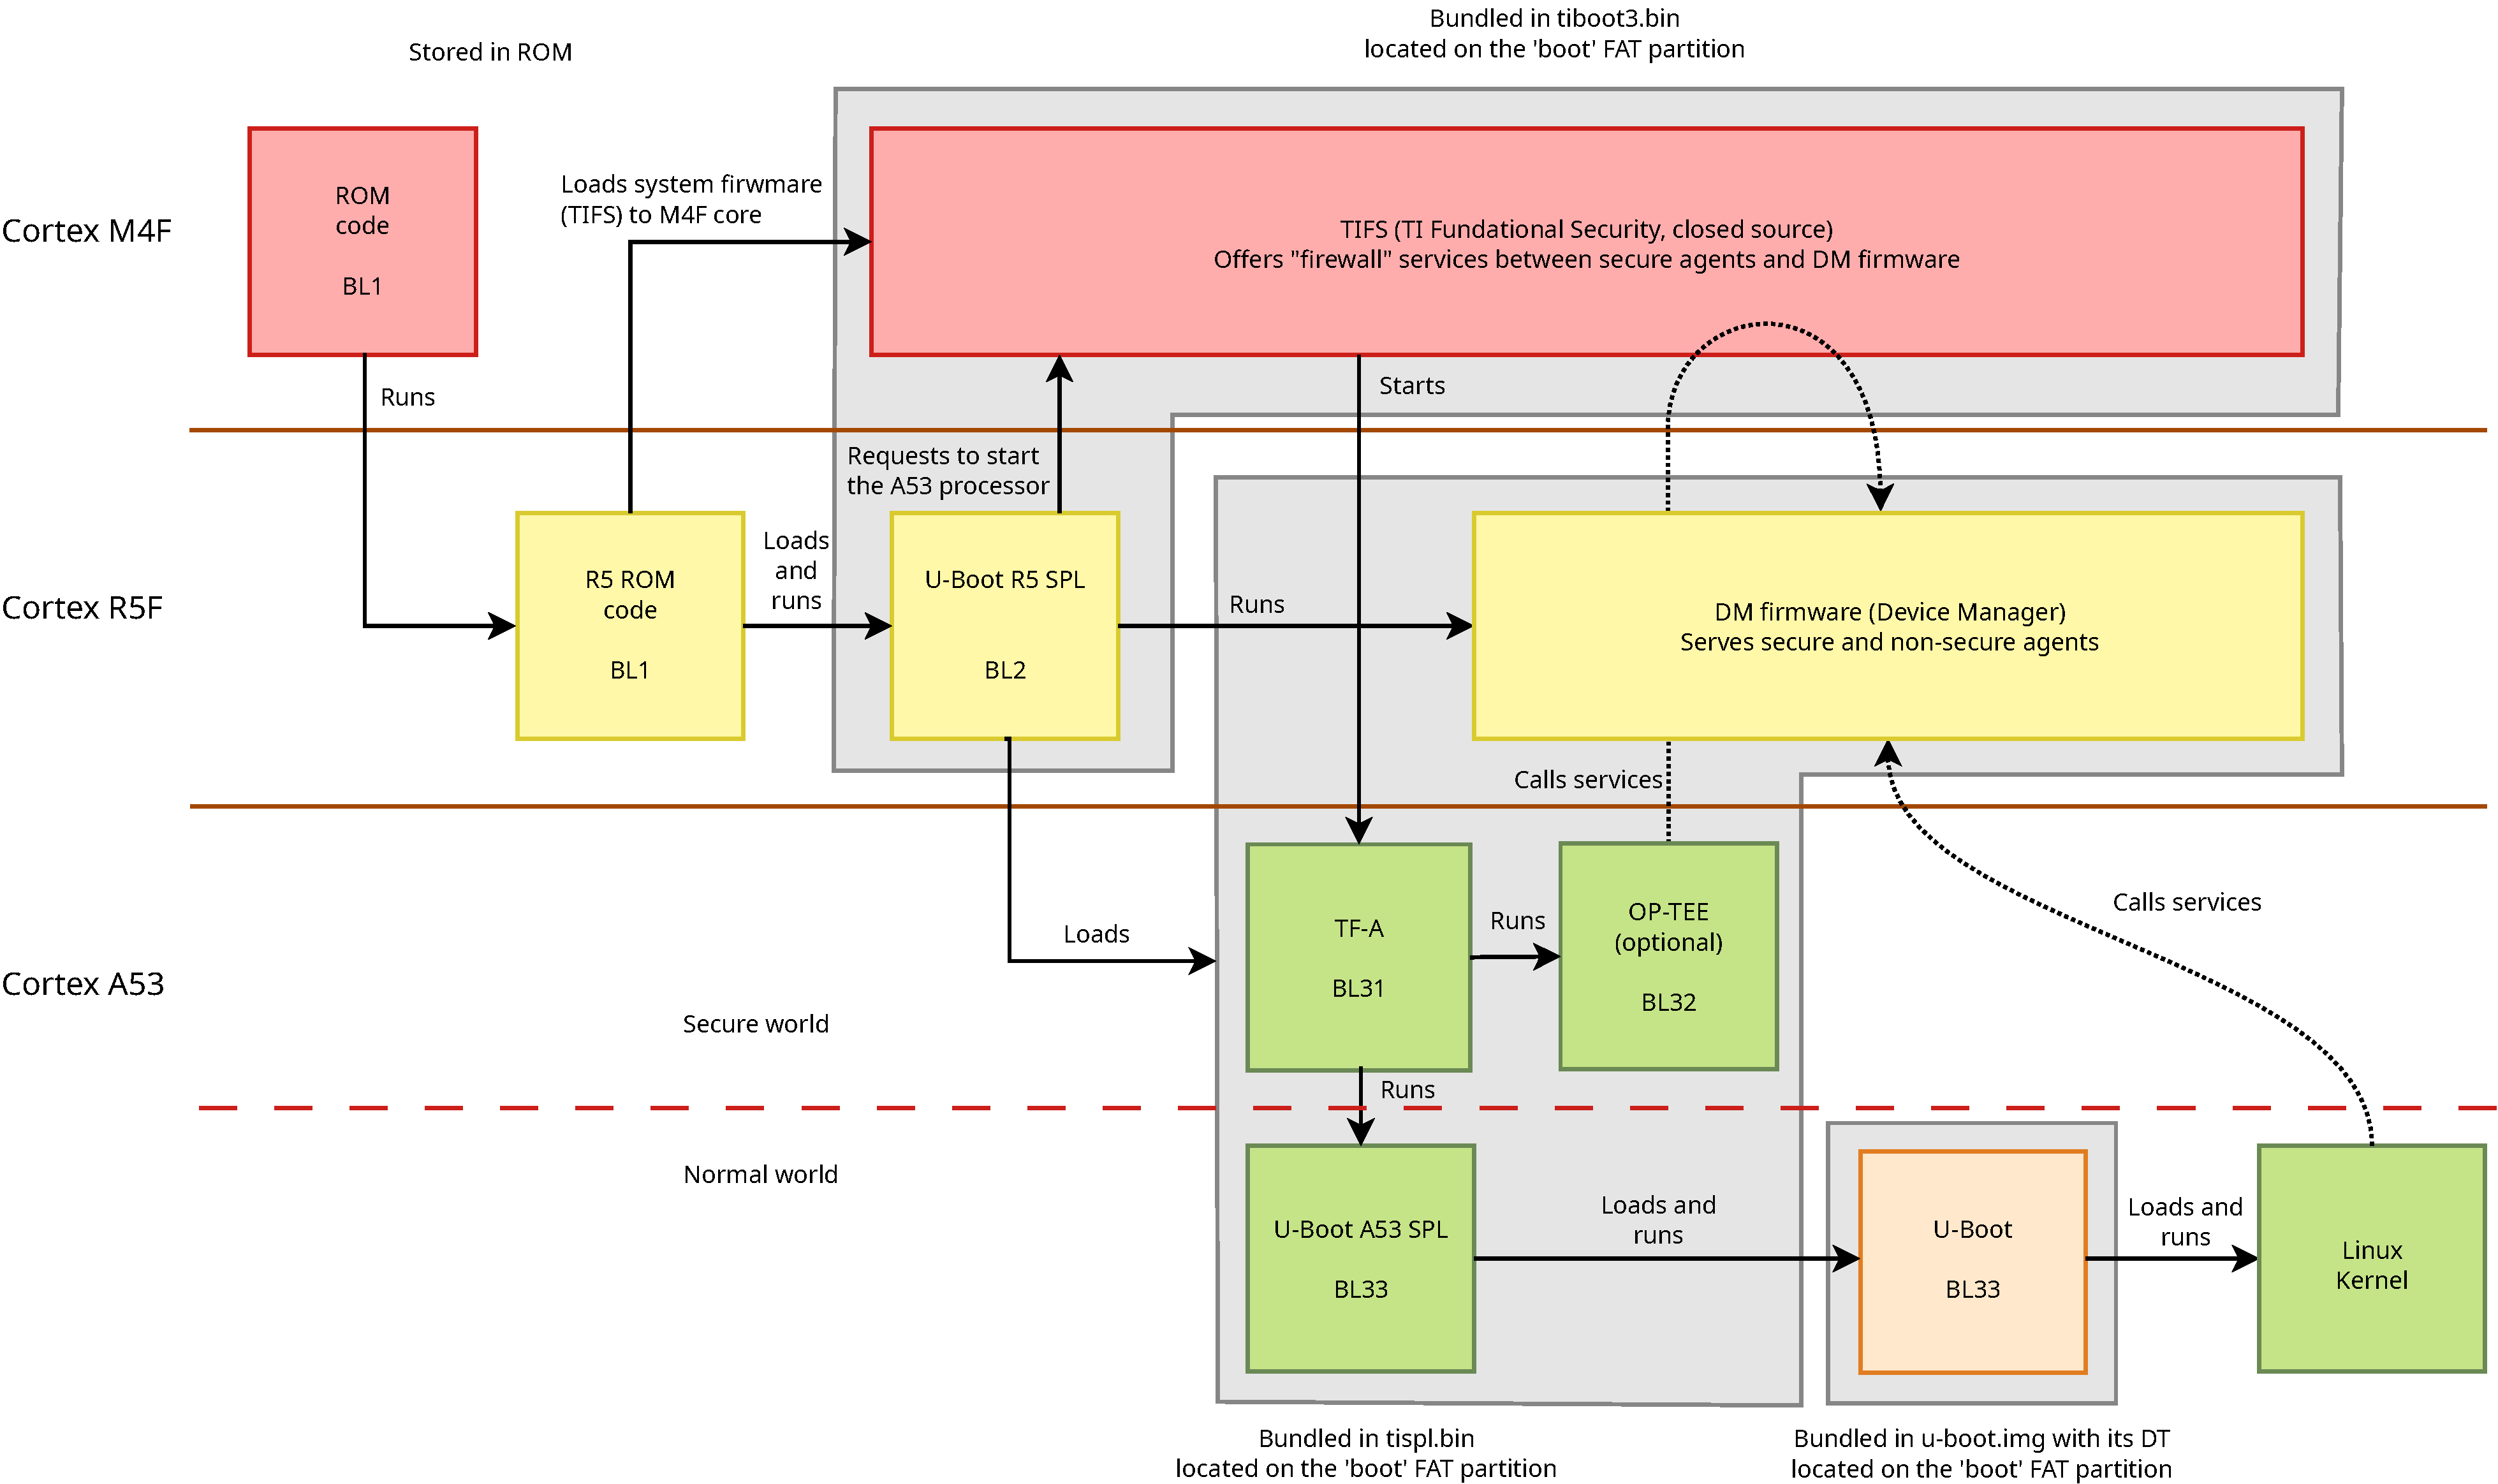
\includegraphics[width=\textwidth]{slides/sysdev-bootloaders-sequence/sequence-am62x.pdf}
  \end{center}
  \\]

